\NeedsTeXFormat{LaTeX2e}

\documentclass[12pt]{article}
\usepackage[letterpaper,portrait, margin=1in]{geometry}
\usepackage{booktabs, pgfplots, bm, multirow, amsmath, wrapfig, gensymb, graphicx}
\pgfplotsset{width=11cm,compat=1.9}
\renewcommand{\arraystretch}{1.5}
\usepackage[colorlinks=true, allcolors=blue]{hyperref}
\usepackage{indentfirst}



\begin{document}
\begin{titlepage}

       %\vspace*{.5cm}
        \begin{center}
        \textbf{\huge PH-291 Physics Lab} \\ 
        \textbf{\Large Professor Corn-Agostini} \\ 
        \textbf{\Large Fall 2022} \\ 
        \vspace*{.5cm}  
        \textbf{\large Lab \# 2: Index of Refraction}
        \vspace{0.5cm}
        \end{center}
       
\noindent Your Name: Perla Berkovitz\\ \\
\noindent Your Lab Section:PH-291-E\\ \\
\noindent Your Lab Instructor: Professor Corn-Agostini\\ \\
\noindent Your Lab Partner's Name: Sharon Sitt\\ \\
\noindent Read and sign Academic Integrity Statement:\\

\noindent {\em I hereby attest that I have not given or received any unauthorized assistance on this assignment.}

    \begin{center}
    \line(1,0){300} \\
    Sign here
    \end{center}

\noindent\textbf{\large Grading Rubric} \\ \\
\renewcommand{\arraystretch}{1.5}
%\large
\begin{tabular}{|l|c|r|l|} 
\hline
 {\bf SECTION } & {\bf POINTS} & {\bf GRADE} & {\bf COMMENTS.................................}\\\hline 
Purpose & 1 & & \\\hline
Data & 3 & & \\\hline
Explanation of Errors & 3 & & \\\hline
Calculations  & 3 & & \\ \hline
Results & 2 & & \\\hline 
Conclusion & 1 & & \\ \hline
Answers & 2 & & \\\hline \hline 
{\em Total} & 15 & & \\ \hline
\end{tabular}

\end{titlepage} 

\newpage
\tableofcontents
\newpage
\section{Purpose}
In this lab, Pfund's Method and Snell's Law will be used to determine the index of refraction of an unknown liquid. 
Two methods will be used to find this index of refraction, the first utilizing Pfund's Method, while the second uses Snell's Law.
The index of refraction of the glass petri dish is determined via Pfund's Method. This then allows us to proceed with both methods. 
As light is refracted through a medium, a small circular region is observed, surrounded by a darker region with a radius that can be used to calculate the unknown index of refraction via Pfund's Law.
In the second method, the incident and reflected angles of the light are measured and plugged into Snell's Law. We can compare the two calculated values to determine the unknown substance.
\newpage
\section{Data}
\begin{center}
    \begin{minipage}{.5\linewidth}
        \centering
        \begin{tabular}{|c | c|}
            \hline
            \textbf{Measurement} & \textbf{Thickness (mm)}  \\ \hline
            1 & 1.695 \\ 
            2 & 1.995 \\ 
            3 & 1.990  \\ 
            4 & 2.095 \\ 
            5 & 1.930 \\ 
            6 & 1.995 \\ \hline
            \multicolumn{2}{|c|}{\textbf{Instrumental Error:} 0.005 mm} \\
            \multicolumn{2}{|c|}{\textbf{Random Error:} 0.055 mm} \\
            \multicolumn{2}{|c|}{\textbf{Thickness:} $1.950\pm0.055$ mm} \\ \hline
        \end{tabular}
        \vspace{3mm}
        \\Table 1: Petri Dish Thickness
        \vspace{10mm}
    \end{minipage}%
    \begin{minipage}{.5\linewidth}
        \centering
        \begin{tabular}{|c | c|}
            \hline
            \textbf{Measurement} & \textbf{Thickness (mm)}  \\ \hline
            1 & 7.98 \\ 
            2 & 8.86 \\ 
            3 & 8.24  \\ 
            4 & 7.60 \\ 
            5 & 8.16 \\ 
            6 & 7.66 \\ \hline
            \multicolumn{2}{|c|}{\textbf{Instrumental Error:} 0.02 mm} \\
            \multicolumn{2}{|c|}{\textbf{Random Error:} 0.19 mm} \\
            \multicolumn{2}{|c|}{\textbf{Thickness:} $8.08\pm0.19$ mm} \\ \hline
        \end{tabular}
        \vspace{3mm}
        \\Table 2: Ring Diameter Without Liquid
        \vspace{10mm}
    \end{minipage} 
    \begin{tabular}{|c|c|}
        \hline
        \textbf{Measurement} & \textbf{Diameter (mm)} \\ \hline
        1 & 19.68 \\ 
        2 & 19.60 \\ 
        3 & 19.58 \\ 
        4 & 19.58 \\ 
        5 & 19.56 \\ 
        6 & 19.62 \\ \hline
        \multicolumn{2}{|c|}{\textbf{Instrumental Error:} 0.02 mm} \\
        \multicolumn{2}{|c|}{\textbf{Random Error:} 0.017 mm} \\
        \multicolumn{2}{|c|}{\textbf{Thickness:} $19.60\pm0.02$ mm} \\ 
        \hline
    \end{tabular}
    \vspace{3mm}
    \\Table 3: Ring Diameter With Liquid
    \begin{tabular}{|c|c c|}
    \hline
        \textbf{Measurement} & \textbf{Incident Angle} & \textbf{Refracted Angle} \\ \hline
        1 & $50.0\degree$ & $28.0\degree$ \\ 
        2 & $28.0\degree$ & $38.0\degree$ \\ 
        3 & $36.0\degree$ & $20.0\degree$ \\ 
        4 & $17.0\degree$ & $40.0\degree$ \\ 
        5 & $43.0\degree$ & $27.0\degree$ \\ 
        6 & $28.0\degree$ & $39.0\degree$ \\ \hline
        \multicolumn{3}{|c|}{\textbf{Instrumental Error:} $0.5\degree$} \\ \hline
    \end{tabular}
    \vspace{3mm}
    \\Table 4: Snell's Law
\end{center}
\newpage
\section{Calculations}
\subsection*{Part A: Pfund's Method}
\noindent \textbf{1. Index of Refraction $\bm{({n_{\textbf{glass}}})}$}\[n_{\textnormal{glass}}=\frac{\sqrt{d^2+16t^2}}{d}\]
    Before the index of refraction of the liquid $(n_\text{liquid})$ could be found, we must first find the index of refraction of our petri dishes $(n_\text{glass})$. Here, $d$ represents the diameter of the ring of light reflected by the glass and $t$ represents the thickness of the petri dish. When solving for $n_\text{glass}$ mean values of $d$ and $t$ were used. The error of the mean values were propagated through this calculation using the following equations. 
\subsubsection*{Error Propagation:}
    \noindent\textbf{1.1 Partial Derivative of Eq. 1 w.r.t $\bm d$}\[\frac{\partial n_{\textnormal{glass}}}{\partial d}=-\dfrac{16t^2}{d^2\sqrt{d^2+16t^2}}\]
    \textbf{1.2 Partial Derivative of Eq. 1 w.r.t $\bm t$} \[\frac{\partial n_{\textnormal{glass}}}{\partial t}=\dfrac{16t}{d\sqrt{16t^2+d^2}}\]
    Each of these partial derivatives are used in the final calculation of the total error associated with $n_\text{glass}.$ Because $d$ and $t$ are both independent variables we use the following equation to find the total error.\\
    \textbf{1.3 Total Error Associated with the Index of Refraction $\bm{({n_{\textbf{glass}}})}$}\[\delta n_{\textnormal{glass}} =\sqrt{\left(\frac{\partial n_{\textnormal{glass}}}{\partial t}\delta t\right)^2+\left(\frac{\partial n_{\textnormal{glass}}}{\partial d}\delta d\right)^2}\]
    The error associated with the mean values were calculated (shown in Table 5). This provides our final error associated with $(n_\text{glass})$.\\
\\\textbf{2. Index of Refraction $\bm{({n_{\textbf{liquid}}})}$}\[n_{\textnormal{liquid}}=\frac{n_{\textnormal{glass}}d}{\sqrt{d^2+16t^2}}\]
    We proceed to calculate $(n_\text{liquid})$, which relies on $(n_\text{glass})$ (calculated above), the diameter $d$ of the first ring reflected by the liquid, and the thickness of the petri dish $t$. The total error of $(n_\text{liquid})$ is found using the following equations.
\subsubsection*{Error Propagation:}
    \noindent\textbf{2.1 Partial Derivative of Eq. 2 w.r.t $\bm d$}\[\frac{\partial n_{\textnormal{liquid}}}{\partial d}=\dfrac{16n_\textnormal{glass}t^2}{\left(d^2+16t^2\right)^\frac{3}{2}}\]
    \textbf{2.2 Partial Derivative of Eq. 2 w.r.t $\bm t$} \[\frac{\partial n_{\textnormal{liquid}}}{\partial t}=-\dfrac{16dn_\text{glass}t}{\left(16t^2+d^2\right)^\frac{3}{2}}\]
    \textbf{2.3 Partial Derivative of Eq. 2 w.r.t $\bm n_\textbf{glass}$}\[\frac{\partial n_{\textnormal{liquid}}}{\partial n_\text{glass}}=\dfrac{d}{\sqrt{16t^2+d^2}}\]
    Each of these partial derivatives are used in calculating the total error in the following equation. All of the variables ($(n_\text{glass}), d, \text{and } t$) are independent, which allows us to use the same process as above (Equation 1.3).\\
    \textbf{2.4 Total Error Associated with the Index of Refraction $\bm{({n_{\textbf{liquid}}})}$}\[\delta n_{\textnormal{liquid}} =\sqrt{\left(\frac{\partial n_{\textnormal{liquid}}}{\partial t}\delta t\right)^2+\left(\frac{\partial n_{\textnormal{liquid}}}{\partial d}\delta d\right)^2+\left(\frac{\partial n_{\textnormal{liquid}}}{\partial n_{\text{glass}}}\delta n_{\text{glass}}\right)^2}\]
    As in Equation 1.3, this equation gives us the total error associated with $(n_\text{liquid})$, shown in the results section (Table 6).
\subsection*{Part B: Snell's Law}
\noindent\textbf{3. The Law of Refraction (Snell's Law)}\[n_1\sin{\theta_1}=n_2\sin{\theta_2}\Rightarrow n_2=\frac{n_1\sin\theta_1}{\sin\theta_2}\]
    Part B of the experiment requires us to employ the Law of Refraction, also known as Snell's Law, to find the index of refraction of the liquid, which we'll refer to as $n_2$. In this equation, $\theta_1$ refers to the incident angle (the angle at which the light enters the medium) and $\theta_2$ refers to the refracted angle (the angle at which the light exits the medium). The final error associated with $n_2$ is given by the following process. 
\subsubsection*{Error Propagation}
\noindent\textbf{3.1 Partial Derivative of Eq. 3 w.r.t $\bm \theta_1$}\[\frac{\partial n_2}{\partial\theta_1}=\dfrac{n_1\cos\left({\theta}_1\right)}{\sin\left({\theta}_2\right)}\]
\textbf{3.2 Partial Derivative of Eq. 3 w.r.t $\bm \theta_2$}\[\frac{\partial n_2}{\partial\theta_2}=-\dfrac{n_1\sin\left({\theta}_1\right)\cos\left({\theta}_2\right)}{\sin^2\left({\theta}_2\right)}\]
    Each of these partial derivatives are used in the following equation to find the total error associated with $n_2$. Because $n_1$ was a given value of the index of refraction of air, there is no error associated with that measurement, so it will not factor into the total error. $\theta_1$ and $\theta_2$ are dependent variables, which allows us to use the following equation to find the total error.\\
\textbf{3.3 Total Error Associated with the Index of Refraction $\bm{({n_{2}})}$}\[\delta n_2= \left|\left(\frac{\partial n_2}{\partial \theta_1}\delta\theta_1\right)\right|+\left|\left(\frac{\partial n_2}{\partial \theta_2}\delta\theta_2\right)\right|\] 
    The total error was calculated using this equation for the measured angles. The mean of the calculated $n_2$ values alongside its error value ($\delta n_2$) provides our final value of the index of refraction of the liquid.\\
\textbf{4. Sample Mean}\[\bar{x}=\frac{\sum\limits^{n}_{i=1}{x_i}}{n}\]
    \begin{center}
        where \(x_i\) represents each value and \(n\) is the total number of entries
    \end{center}
\textbf{5. Sample Standard Deviation}\[S_x^2=\frac{1}{N_x-1}\sum^{N_x}_{i=1}(x_i-\bar{x})^2 \]
    \begin{center}
        where \(S_x^2\) is the sample variance and \(S_x\) is the sample standard deviation for each sample set. \(N_x\) is the number of samples in the set. \\
    \end{center}
\textbf{6. Standard Deviation of the Mean (SDOM)}\[\sigma_x=\frac{S_x}{\sqrt{N_x}}\]
    \begin{center}
        This also provides us with the random error of each sample set.\\
    \end{center}
\newpage
\section{Results}
\begin{center}
    \centering
    \begin{tabular}{|c|c|c|c|}
    \hline
        $n_\text{glass}$ & $\frac{\partial n_\text{glass}}{\partial t}$ & $\frac{\partial n_\text{glass}}{\partial d}$ & Error of $n_\text{glass}$ \\ \hline
        1.39 & 0.34 & -0.08 & 0.08 \\ \hline
        \multicolumn{4}{|c|}{$\bm{n_\textbf{glass}: 1.39\pm0.08}$}\\\hline
    \end{tabular}
    \vspace{3mm}
    \\ Table 5: $n_\text{glass}$ Final Value by Pfund's Method\\
    \vspace{5mm}
    \centering
    \begin{tabular}{|c|c|c|c|c|c|}
    \hline
        $n_\text{liquid}$ & $\frac{\partial n_\text{liquid}}{\partial t}$ & $\frac{\partial n_\text{liquid}}{\partial d}$ & $\frac{\partial n_\text{liquid}}{\partial n_{\text{glass}}}$ & Error of $n_\text{glass}$ & Error of $n_\text{liquid}$ \\ \hline
        1.29 & -0.09 & 0.009 & 0.93 & 0.08 & 0.26 \\ \hline
        \multicolumn{6}{|c|}{$\bm{n_\textbf{liquid}: 1.29\pm0.26}$}\\\hline
    \end{tabular} 
    \vspace{3mm}
    \\ Table 6: $n_\text{liquid}$ Final Value by Pfund's Method\\
    \vspace{5mm} 
    \centering
    \begin{tabular}{|c|c|c|c|}
    \hline
        $n_\text{liquid}$ & $\frac{\partial n_\text{liquid}}{\partial \theta_1}$ & $\frac{\partial n_\text{liquid}}{\partial \theta_2}$  & Error of $n_\text{liquid}$ \\ \hline
        1.62 & 1.88 & -3.82 & 0.04  \\ \hline
        \multicolumn{4}{|c|}{$\bm{n_\textbf{liquid}: 1.62\pm0.04}$}\\\hline
    \end{tabular} 
    \vspace{3mm}
    \\ Table 7: $n_\text{liquid}$ Final Value by Snell's Law\\
    \vspace{5mm}
    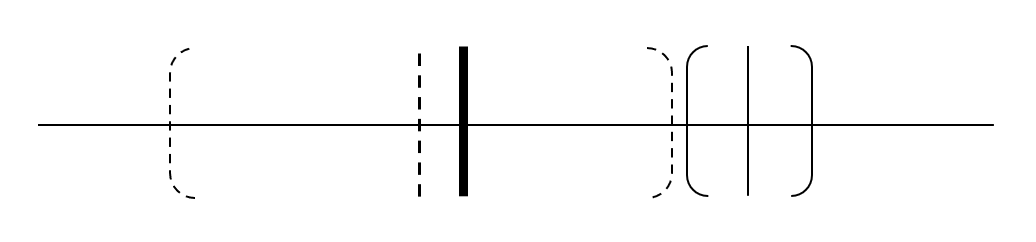
\includegraphics[scale=0.5]{number line.png}\\
    Dashed = Method 1 (Pfund's Method)\\
    Solid = Method 2 (Snell's Law)\\
    Bold = Accepted Value \\
    Figure 1: Number Line Indicating Error Bounds and Accepted Values   
\end{center}
Using Figure 1, we can see that while the index of refraction calculated via Pfund's Method had a greater error, it was closer to the accepted value of the index of refraction of water, which is 1.33. The accepted index of refraction lies within the error bounds of the Pfund's Method calculation. Snell's method provided an index of refraction of $1.62\pm0.04$ which does not agree with the accepted value. This can mainly be attributed to human error in measuring the incident and refracted angles. When measuring our angles, we misread our protractor as having increments at every $1\degree$, as opposed to every $0.5\degree$. This provided us with an instrumental error of $0.5\degree$, as opposed to $0.25\degree$.
\\\indent The error introduced in Pfund's Method stems from multiple areas. Firstly, the petri dish may not have had a uniform thickness, providing different thickness readings on the micrometer. Then, the laser may not have been pointed perfectly vertically. Pfund's method relies on the laser making an angle of $\frac{\pi}{2}$ with the horizontal. Lastly, error is introduced in measuring each of the rings. The method of measuring required eyeballing where the ring lined up on the polar grid and then measuring the polar grid on a separate piece of paper. Measurements were taken using a pair of vernier calipers, which have pointed ends where the measurements are taken. These tended to make indentations in the polar grid paper which the calipers would slide into when taking other measurements.\\
\indent The second method using Snell's Law had less error associated with the final index of refraction relative to the value found by Pfund's Method. The calculated index of refraction is $1.62\pm0.04$. While tracing the petri dish onto our surface, the polar grid on the bottom of the dish caused us to trace a larger circle than the diameter of the petri dish. Then, when placing the pins along the path of the laser, the laser may have been nudged out of position. This would affect the accuracy of our measured angles. The center of the circle may also have been misplaced, as it is found using the perpendicular bisectors of two cords. These perpendicular bisectors may not have been exactly perpendicular. This would affect the measurements taken for our angles, and in turn affect our index of refraction.
\newpage
\section{Conclusion}
Using Pfund's Method, an index of refraction of $1.29\pm0.26$ was calculated. The accepted value of the index of refraction is 1.33, which lies within the error bound of the value calculated via Pfund's Method. However, when directly applying Snell's Law, the index of refraction is found to be $1.62\pm0.03$, which does not match the accepted value. While this method was more precise than Pfund's Method (error of $\pm0.03$ as opposed to $\pm0.26$), the values calculated via Pfund's Method were more accurate (0.04 less than the accepted value). The significant difference between final values can be directly attributed to human error, as described in the previous section. 
Given that Pfund's Method is an application of Snell's Law, both methods should produce similar results if error can be further reduced.
\newpage
\section{Questions}
\subsection*{1. Derive the equation for $\bm n_\text{glass}$ and include the derivation in your report.}
    Let $d$ be the diameter of the circle bordering the grey region, $t$ be the thickness of the glass petri dish, and $\theta_c$ be the critical angle. Let us begin with Snell's Law.
    \[n_1\sin{\theta_1}=n_2\sin{\theta_2}\rightarrow n_{\text{glass}}\sin{\theta_c}=n_{\text{air}}\sin{\frac{\pi}{2}}\]
    \[n_{\text{glass}}=\frac{n_{\text{air}}}{\sin\theta_c}=\frac{1}{\sin\theta_c}=\frac{\text{Hypotenuse}}{\text{Opposite}}\]
    \[n_{\text{glass}}=\frac{\sqrt{\left(\frac{d}{4}\right)^2+t^2}}{\frac{d}{4}}=\frac{4\sqrt{\frac{d^2}{16}+t^2}}{d}=\frac{\sqrt{16\left(\frac{d^2}{16}\right)+t^2}}{d}=\frac{\sqrt{d^2+16t^2}}{d}\]
\subsection*{2. Derive the equation for $\bm n_{\text{liquid}}$ and include the derivation in your report.}
    Let $d_{\text{liquid}}$ be the diameter of the larger dark ring, $t$ be the thickness of the glass petri dish, and $\theta_c$ be the critical angle. Let us begin with Snell's Law.
    \[n_{\text{glass}}\sin{\theta_c}=n_{\text{liquid}}\sin{\frac{\pi}{2}}\rightarrow n_{\text{glass}}\sin\theta_c=n_{\text{liquid}}\]
    \[n_{\text{glass}}\sin{\theta_c}=n_{\text{glass}}\left[\frac{\frac{d_{\text{liquid}}}{4}}{\sqrt{\left(\frac{d_{\text{liquid}}}{4}\right)^2+t^2}}\right]=n_{\text{glass}}\frac{d_{\text{liquid}}}{4\sqrt{\left(\frac{d^2_\text{liquid}}{16}\right)+t^2}}=\frac{n_{\text{glass}}d_{\text{liquid}}}{\sqrt{16\left(\frac{d_{\text{liquid}}^2}{16}\right)+t^2}}\]
    \[n_{\text{liquid}}=\frac{n_{\text{glass}}d_\text{liquid}}{\sqrt{d^2_{\text{liquid}}+16t^2}}\]
\subsection*{3. What assumptions or approximations, if any, have been made in the Snell's Law technique? Do you think it/they were reasonable ones? Support your answer quantitatively.}
    In the Snell's Law technique, multiple assumptions were made. First, the water is assumed to be pure, so that no particles would affect the reflection of light and in turn the index of refraction. Another assumption made is that the pins are placed accurately enough to recreate the angles of incidence and refraction. All instruments, like the protractor, are assumed to be accurate and laid properly on the surface. The laser and protractor are assumed to be laid perfectly flat and have not moved throughout the experiment.
    Although the value for the index of refraction calculated using this method ($1.62 \pm 0.03$) does not match with the accepted value for the index of refraction (1.33), these assumptions are still considered to be reasonable. Because of the significant human error present in the experiment, in particular in the Snell's Law technique, the approximations associated with the experiment are reasonable.
\subsection*{4. Will Pfund’s method work for liquids of all $n$? Explain.}
    Pfund's Method will not work if the index of refraction for the liquid is larger than the index of refraction for the glass. The sine of an angle cannot exceed 1, and such \[\sin\theta_c=\frac{n_{\text{liquid}}}{n_{\text{glass}}}\le 1\]
    If the value of $n_{\text{glass}}$ is smaller than the value of $n_{\text{liquid}}$, the value of $\sin\theta_c$ would exceed 1, which is impossible. No critical angle ($\theta_c$) could exist, and in turn, there would be no total internal reflection and no rings appearing.
\end{document}